\begin{frame}
    \frametitle{Artificial Intelligence}

    \begin{itemize}
        \item hard to define, since intelligence itself is precisely defined
        \item ``Artificial intelligence leverages computers and machines to mimic the problem-solving and decision-making capabilities of the human mind.''
        \item distinction: strong and weak AI
        \begin{itemize}
            \item strong: generic AI that can solve generic issues
            \item weak/narrow: for one specific issue
        \end{itemize}
    \end{itemize}

    \begin{figure}
        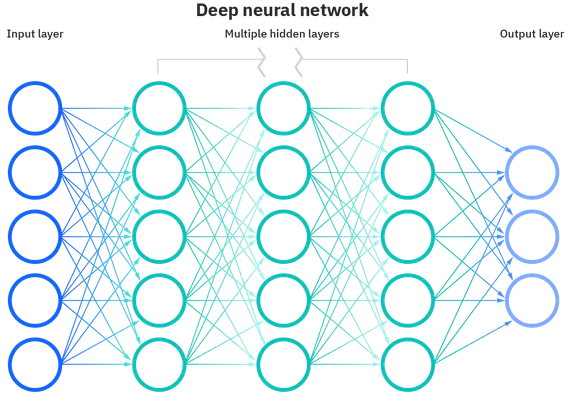
\includegraphics[height=.3\textheight]{dnn}
        \caption{Deep Neuronal Network}
        \label{fig:dnn}
    \end{figure}
\end{frame}

\begin{frame}
    \frametitle{Terminology}
    \textbf{Deep Learning}
    is essentially an autonomous, self-teaching system in which you use existing data to train algorithms
    to find patterns and then use that to make predictions about new data.

    \textbf{Reinforcement Learning}
    \begin{itemize}
        \item is an autonomous, self-teaching system that essentially learns by trial and error
        \item performs actions with the aim of maximizing rewards, or in other words: learning by doing
    \end{itemize}

    \frametitle{Deep Learning vs. Reinforcement Learning}
    \begin{itemize}
        % The difference between them is that deep learning is learning from a training set and then applying that
        % learning to a new data set, while reinforcement learning is dynamically learning by adjusting actions based
        % in continuous feedback to maximize a reward.
        \item are both systems that learn autonomously.
        % In fact, you might use deep learning in a reinforcement learning system, which is referred to as deep
        % reinforcement learning
        \item aren’t mutually exclusive.
    \end{itemize}
\end{frame}

\begin{frame}
    \frametitle{Markow Decision Process}
    A Markov decision process is a 4-tuple $(S,A,P_{a},R_{a})$, where:

    \begin{itemize}
        \item $S$ is a set of states called the state space,
        \item $A$ is a set of actions called the action space (alternatively, $A_s$ is the set of actions available from state $s$),
        \item $P_{a}(s,s')=\Pr(s_{t+1}=s'\mid s_{t}=s,a_{t}=a)$ is the probability that action a in state s at time $t$ will lead to state s' at time $t+1$,
        \item $R_{a}(s,s')$ is the immediate reward (or expected immediate reward) received after transitioning from state $s$ to state $s'$, due to action $a$
        \item $S$ is a set of states
    \end{itemize}

    Optimizing for highest reward

    % Machine-Learning-Konzept bei dem ohne Kontextinformationen oder Wissen über Handlungskonsequenzen trainiert wird. Ziel: Maximale Belohnung
    % Durch viel probieren wird gelernt, welcher Pfad zur Lösung führt (verstärkt/belohnt) bzw welcher nicht (geschwächt, bestraft)
\end{frame}

\begin{frame}
    \frametitle{Algorithms}

    \begin{itemize}
        \item DMC: Deep Monte Carlo
        \item DQN: Deep Q-Network
        \item NFSP: Neural Fictitious Self-Play
        \item CFR: Counterfeit Regret Minimization
    \end{itemize}
\end{frame}
